\documentclass{standalone}
\usepackage[utf8]{inputenc}
\usepackage{pgfplots}
\DeclareUnicodeCharacter{2212}{−}
\usepgfplotslibrary{groupplots,dateplot}
\usetikzlibrary{patterns,shapes.arrows}
\pgfplotsset{compat=newest}
\begin{document}
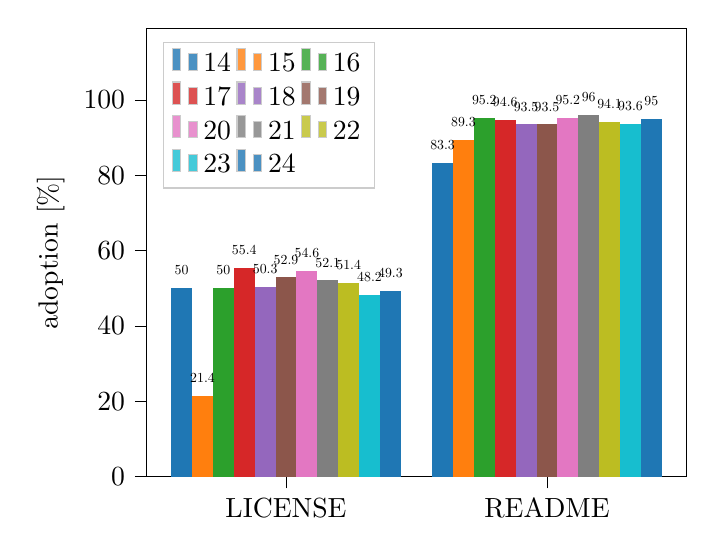
\begin{tikzpicture}

\definecolor{crimson2143940}{RGB}{214,39,40}
\definecolor{darkgray176}{RGB}{176,176,176}
\definecolor{darkorange25512714}{RGB}{255,127,14}
\definecolor{darkturquoise23190207}{RGB}{23,190,207}
\definecolor{forestgreen4416044}{RGB}{44,160,44}
\definecolor{goldenrod18818934}{RGB}{188,189,34}
\definecolor{gray127}{RGB}{127,127,127}
\definecolor{lightgray204}{RGB}{204,204,204}
\definecolor{mediumpurple148103189}{RGB}{148,103,189}
\definecolor{orchid227119194}{RGB}{227,119,194}
\definecolor{sienna1408675}{RGB}{140,86,75}
\definecolor{steelblue31119180}{RGB}{31,119,180}

\begin{axis}[
legend cell align={left},
legend columns=3,
legend style={
  fill opacity=0.8,
  draw opacity=1,
  text opacity=1,
  at={(0.03,0.97)},
  anchor=north west,
  draw=lightgray204
},
tick align=outside,
tick pos=left,
x grid style={darkgray176},
xmin=-0.454, xmax=1.614,
xtick style={color=black},
xtick={0.08,1.08},
xticklabels={LICENSE,README},
y grid style={darkgray176},
ylabel={adoption [\%]},
ymin=0, ymax=119,
ytick style={color=black}
]
\draw[draw=none,fill=steelblue31119180] (axis cs:-0.36,0) rectangle (axis cs:-0.28,50);
\addlegendimage{ybar,ybar legend,draw=none,fill=steelblue31119180}
\addlegendentry{14}

\draw[draw=none,fill=steelblue31119180] (axis cs:0.64,0) rectangle (axis cs:0.72,83.3);
\draw[draw=none,fill=darkorange25512714] (axis cs:-0.28,0) rectangle (axis cs:-0.2,21.4);
\addlegendimage{ybar,ybar legend,draw=none,fill=darkorange25512714}
\addlegendentry{15}

\draw[draw=none,fill=darkorange25512714] (axis cs:0.72,0) rectangle (axis cs:0.8,89.3);
\draw[draw=none,fill=forestgreen4416044] (axis cs:-0.2,0) rectangle (axis cs:-0.12,50);
\addlegendimage{ybar,ybar legend,draw=none,fill=forestgreen4416044}
\addlegendentry{16}

\draw[draw=none,fill=forestgreen4416044] (axis cs:0.8,0) rectangle (axis cs:0.88,95.2);
\draw[draw=none,fill=crimson2143940] (axis cs:-0.12,0) rectangle (axis cs:-0.04,55.4);
\addlegendimage{ybar,ybar legend,draw=none,fill=crimson2143940}
\addlegendentry{17}

\draw[draw=none,fill=crimson2143940] (axis cs:0.88,0) rectangle (axis cs:0.96,94.6);
\draw[draw=none,fill=mediumpurple148103189] (axis cs:-0.04,0) rectangle (axis cs:0.04,50.3);
\addlegendimage{ybar,ybar legend,draw=none,fill=mediumpurple148103189}
\addlegendentry{18}

\draw[draw=none,fill=mediumpurple148103189] (axis cs:0.96,0) rectangle (axis cs:1.04,93.5);
\draw[draw=none,fill=sienna1408675] (axis cs:0.04,0) rectangle (axis cs:0.12,52.9);
\addlegendimage{ybar,ybar legend,draw=none,fill=sienna1408675}
\addlegendentry{19}

\draw[draw=none,fill=sienna1408675] (axis cs:1.04,0) rectangle (axis cs:1.12,93.5);
\draw[draw=none,fill=orchid227119194] (axis cs:0.12,0) rectangle (axis cs:0.2,54.6);
\addlegendimage{ybar,ybar legend,draw=none,fill=orchid227119194}
\addlegendentry{20}

\draw[draw=none,fill=orchid227119194] (axis cs:1.12,0) rectangle (axis cs:1.2,95.2);
\draw[draw=none,fill=gray127] (axis cs:0.2,0) rectangle (axis cs:0.28,52.1);
\addlegendimage{ybar,ybar legend,draw=none,fill=gray127}
\addlegendentry{21}

\draw[draw=none,fill=gray127] (axis cs:1.2,0) rectangle (axis cs:1.28,96);
\draw[draw=none,fill=goldenrod18818934] (axis cs:0.28,0) rectangle (axis cs:0.36,51.4);
\addlegendimage{ybar,ybar legend,draw=none,fill=goldenrod18818934}
\addlegendentry{22}

\draw[draw=none,fill=goldenrod18818934] (axis cs:1.28,0) rectangle (axis cs:1.36,94.1);
\draw[draw=none,fill=darkturquoise23190207] (axis cs:0.36,0) rectangle (axis cs:0.44,48.2);
\addlegendimage{ybar,ybar legend,draw=none,fill=darkturquoise23190207}
\addlegendentry{23}

\draw[draw=none,fill=darkturquoise23190207] (axis cs:1.36,0) rectangle (axis cs:1.44,93.6);
\draw[draw=none,fill=steelblue31119180] (axis cs:0.44,0) rectangle (axis cs:0.52,49.3);
\addlegendimage{ybar,ybar legend,draw=none,fill=steelblue31119180}
\addlegendentry{24}

\draw[draw=none,fill=steelblue31119180] (axis cs:1.44,0) rectangle (axis cs:1.52,95);
\draw (axis cs:-0.32,50) ++(0pt,3pt) node[
  scale=0.5,
  anchor=south,
  text=black,
  rotate=0.0
]{50};
\draw (axis cs:0.68,83.3) ++(0pt,3pt) node[
  scale=0.5,
  anchor=south,
  text=black,
  rotate=0.0
]{83.3};
\draw (axis cs:-0.24,21.4) ++(0pt,3pt) node[
  scale=0.5,
  anchor=south,
  text=black,
  rotate=0.0
]{21.4};
\draw (axis cs:0.76,89.3) ++(0pt,3pt) node[
  scale=0.5,
  anchor=south,
  text=black,
  rotate=0.0
]{89.3};
\draw (axis cs:-0.16,50) ++(0pt,3pt) node[
  scale=0.5,
  anchor=south,
  text=black,
  rotate=0.0
]{50};
\draw (axis cs:0.84,95.2) ++(0pt,3pt) node[
  scale=0.5,
  anchor=south,
  text=black,
  rotate=0.0
]{95.2};
\draw (axis cs:-0.08,55.4) ++(0pt,3pt) node[
  scale=0.5,
  anchor=south,
  text=black,
  rotate=0.0
]{55.4};
\draw (axis cs:0.92,94.6) ++(0pt,3pt) node[
  scale=0.5,
  anchor=south,
  text=black,
  rotate=0.0
]{94.6};
\draw (axis cs:0,50.3) ++(0pt,3pt) node[
  scale=0.5,
  anchor=south,
  text=black,
  rotate=0.0
]{50.3};
\draw (axis cs:1,93.5) ++(0pt,3pt) node[
  scale=0.5,
  anchor=south,
  text=black,
  rotate=0.0
]{93.5};
\draw (axis cs:0.08,52.9) ++(0pt,3pt) node[
  scale=0.5,
  anchor=south,
  text=black,
  rotate=0.0
]{52.9};
\draw (axis cs:1.08,93.5) ++(0pt,3pt) node[
  scale=0.5,
  anchor=south,
  text=black,
  rotate=0.0
]{93.5};
\draw (axis cs:0.16,54.6) ++(0pt,3pt) node[
  scale=0.5,
  anchor=south,
  text=black,
  rotate=0.0
]{54.6};
\draw (axis cs:1.16,95.2) ++(0pt,3pt) node[
  scale=0.5,
  anchor=south,
  text=black,
  rotate=0.0
]{95.2};
\draw (axis cs:0.24,52.1) ++(0pt,3pt) node[
  scale=0.5,
  anchor=south,
  text=black,
  rotate=0.0
]{52.1};
\draw (axis cs:1.24,96) ++(0pt,3pt) node[
  scale=0.5,
  anchor=south,
  text=black,
  rotate=0.0
]{96};
\draw (axis cs:0.32,51.4) ++(0pt,3pt) node[
  scale=0.5,
  anchor=south,
  text=black,
  rotate=0.0
]{51.4};
\draw (axis cs:1.32,94.1) ++(0pt,3pt) node[
  scale=0.5,
  anchor=south,
  text=black,
  rotate=0.0
]{94.1};
\draw (axis cs:0.4,48.2) ++(0pt,3pt) node[
  scale=0.5,
  anchor=south,
  text=black,
  rotate=0.0
]{48.2};
\draw (axis cs:1.4,93.6) ++(0pt,3pt) node[
  scale=0.5,
  anchor=south,
  text=black,
  rotate=0.0
]{93.6};
\draw (axis cs:0.48,49.3) ++(0pt,3pt) node[
  scale=0.5,
  anchor=south,
  text=black,
  rotate=0.0
]{49.3};
\draw (axis cs:1.48,95) ++(0pt,3pt) node[
  scale=0.5,
  anchor=south,
  text=black,
  rotate=0.0
]{95};
\end{axis}

\end{tikzpicture}

\end{document}
